\section{Modello del Big Bang}\label{sec:big-bang}
\subsection{Età e Confini dell'universo}\label{sec:eta-confini-universo}

Se è vero che il nostro universo si sta espandendo, questo vuol dire che andando indietro col tempo, le galassie dovessero essere decisamente più vicine tra loro, fino a che all'origine di tutto lo spazio-tempo dovesse essere racchiuso in uno spazio puntiforme. Questa è la serie di ragionamenti che hanno portato alla deduzione della teoria del \textit{Big Bang}. Siccome prima dell'evento che ha scatenato l'espansione, non ha senso parlare di tempo e spazio, allora facciamo coincidere l'origine del tempo con il Big Bang, perciò si ha che l'età dell'universo coincide con il tempo passato da esso.

Si è calcolato che il tempo necessario per far si che le galassie si allontanassero della distanza $d$ che osserviamo oggi alla di recessione $v$ dovuta all'espansione dell'universo (approssimando $v$ costante per semplicità), ci restituisce l'età dell'universo. Se $d = v t_H$, allora:
\[
    v = H_0 v t_H
\]
\begin{equation} \label{eq:eta-universo}
    t_H \equiv \frac{1}{H_0} \simeq \frac{1}{\SI{73}{km.s^{-1}.Mpc^{-1}}} = \frac{\SI{1}{Mpc}}{\SI{73}{km}} = \frac{\SI{3.1e19}{km}}{\SI{73}{km}} = \SI{13.4e9}{yr}
\end{equation}
In realtà le ultime stime di tale valore lo portano vicino a $\SI{13.7e9}{yr}$.

Conoscendo questo valore e sapendo che la velocità massima raggiungibile all'interno dell'universo è $c$, allora si può stimare la dimensione della bolla di universo osservabile, cioè quella porzione di spazio-tempo è possibile osservare al massimo, fissato un sistema di riferimento.
\[
    d_H \sim c t_H \sim \SI{4000}{Mpc}
\]

Prima del Big Bang il punto materiale in cui era concentrato tutto lo spzio-tempo, definito con il termine \textit{Sincolarità Cosmica}, aveva temperatura e densità che tendevano all'infinito e a causa di ciò, non è possibile studiare nulla nei primi $t_p = \SI{5.39e-44}{s}$ della sua vita. Questo valore viene detto \textit{tempo di Planck} ($t_P$) e si tratta del tempo che impiega la luce a percorre una \textit{lunghezza di Planck} ($d_P = \sim \SI{e-33}{cm}$)

\subsection{Un universo in Espansione}\label{sec:unverso-espansione}
Non appena dopo il Big Bang l'universo si trovava in uno stato estremamente denso di plasma molto caldo che emetteva radiazione termica, questa radiazione è quella che viene osservata oggi sotto forma di \textit{Cosmic Microwave Background (CMB)}. Tale radiazione, chiamata anche radiazione fossile, sarebbe dovuta essere a spettro continuo, simile a quello di un corpo nero, ma soprattutto, se vere le ipotesi di uniformità e isotropia, sarebbe dovuta essere uniforme su tutta la volta celeste. 

Le osservazioni mostrarono proprio un universo estremamente isotropo e uniforme in tutte le direzioni, insieme ad avere uno spettro che segue perfettamente quello di un corpo nero a temperatura $T = \SI{2.725}{K}$, come mostra il grafico in figura~\ref{fig:balckbody-universe}. tale radiazione è stata emessa ad un redshift $z \sim 1100$ da un plasma ad una temperatura di $T \sim \SI{3000}{K}$.
\begin{figure}
    \centering
    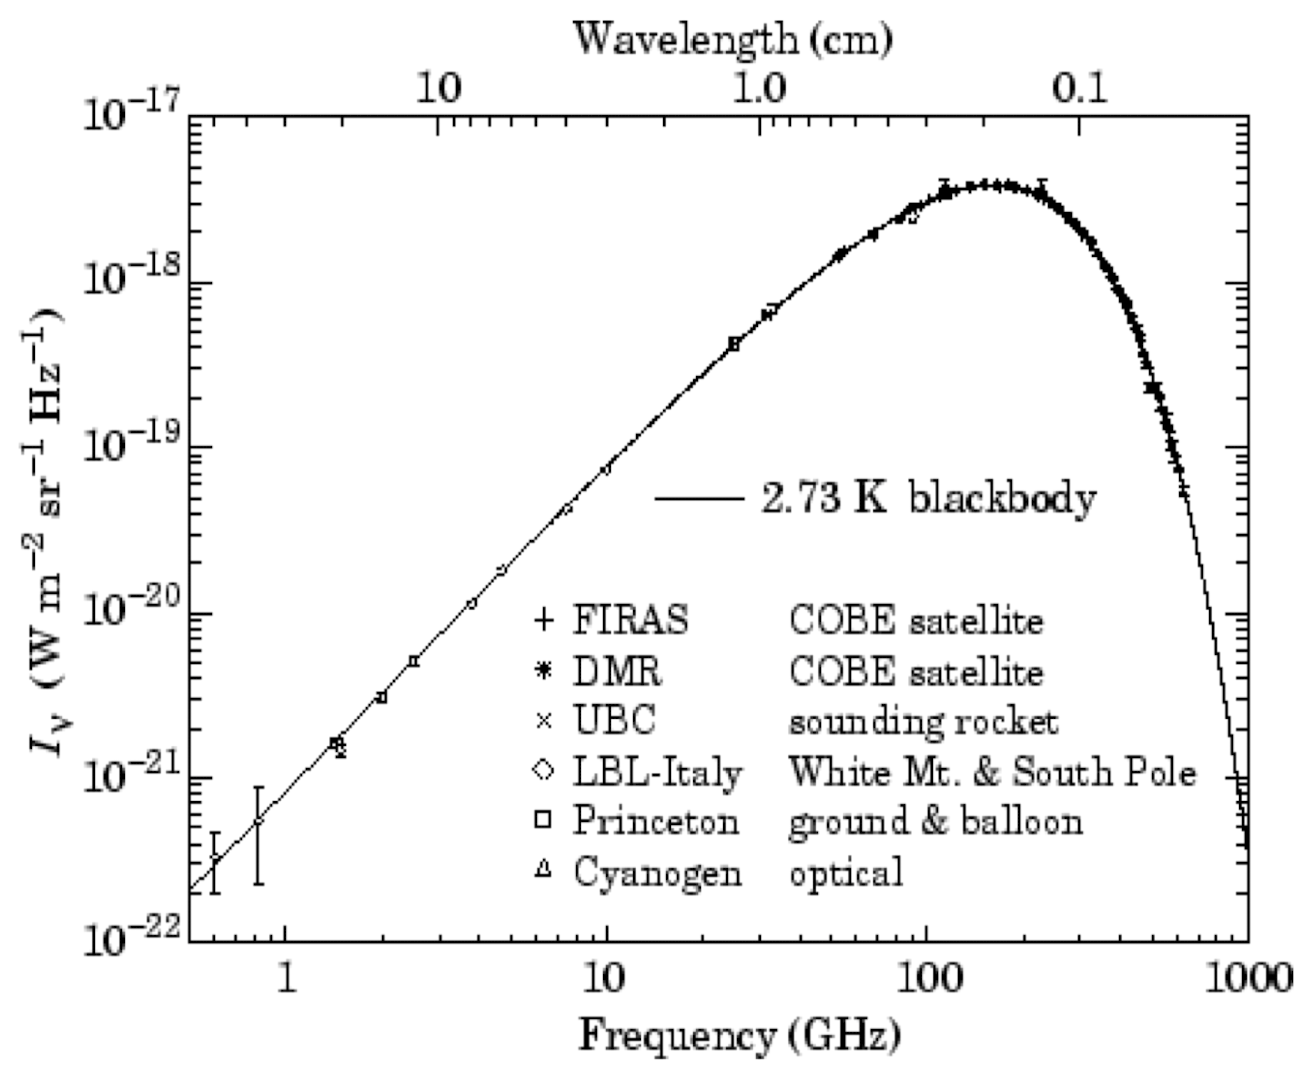
\includegraphics[width = 0.5\textwidth]{immagini/blackbody-universe.png}
    \caption{La figura mostra l'andamento dello spettro della radiazione proveniente dal CMB comparato con quello di un corpo nero. Dalla legge di Wien (\refeq{eq:legge-wien}) si osserva che $\lambda_{max}= \SI{0.11}{cm}$}\label{fig:balckbody-universe}
\end{figure}

Al fine di descrivere un universo in espansione che rispetti le condizioni cosmologiche risulta conveniente introdurre dei concetti cardine. In particolare:
\begin{description}
    \item[unicità della coordinata temporale t], grazie alla simmetria implicita all'interno dei principi, questa risulta comoda per catalogare i vari eventi cosmologici;
    \item[osservatore in comovimento], ovvero in quiete rispetto all'espansione dell'universo;
    \item[distanza in comovimento (x)], ovvero la distanza tra due osservatori in quiete rispetto all'espansione dell'universo è costante rispetto al tempo;
    \item[distanza propria (r)], definita come $r(t) = x R(t)$, tra due osservatori in quiete rispetto all'espansione, varia in funzione del tempo;
    \item[fattore di scala cosmico $R(t)$], si tratta di una funzione adimensionale del tempo, la quale descrive l'espansione dello spazio tempo.
\end{description}

Un'assunzione comune è la normalizzazione di tale fattore di scala, imponendo che al tempo presente ($t_0$) questa sia unitaria,
\[
    R(t_0) = R_0 = 1
\]
il che vuol dire che oggi la distanza in comovimento tra due osservatori in quiete rispetto all'espansione dello spaziotempo equivale alla loro distanza propria ($x = r(t_0) = r_0$), per cui si può esprimere la distanza propria come:
\[
    r(t)= r_0 R(t)
\]

La distanza tra due osservatori in comovimento separati da $r(t)$ ad un dato istante di tempo sarà perciò:
\begin{equation}\label{eq:hubble-speed}
    v(t) = \dot{r}(t) = r_0 \dot{R}(t) = \frac{\dot{R}(t)}{R(t)}r(t)
\end{equation}

Utilizzando la relazione~\refeq{eq:hubble} di Hubble, si ottiene una stima del parametro H in funzione del tempo.
\[
    v(t) = H(t)r(t)
\]
\begin{equation}\label{eq:hubble-scale}
    H(t) = \frac{\dot{R}(t)}{R(t)}
\end{equation}
Per cui la costante di Hubble è una misura del tasso di espansione dell'universo.

Infine esiste una relazione tra il fattore di scala cosmico e il redshift, presa infatti la lunghezza d'onda della radiazione proveniente da un corpo, lo spostamento vero il rosso è dovuto all'espansione dello spazio-tempo che la allunga. Sia $\lambda_{em} = \lambda_0 R(t_{em})$ la lunghezza d'onda al momento dell'emissione e $\lambda_{obs} = \lambda_0 R_0 = \lambda_0$ quella osservata oggi. Allora, dall'equazione~\refeq{eq:redshift} per il redshift,
\[
    z = \frac{\lambda_0}{\lambda_0 R(t)}-1
\]
ottenendo l'equazione~\refeq{eq:redshift-rescale}
\begin{equation}\label{eq:redshift-rescale}
    z + 1 = \frac{1}{R(t)} 
\end{equation}